\chapter{Lokalisation}

\section{Lokalisatonsumgebung/\red[Karte]}
\label{chap.map}
Die Bestimmung der Pose des \kps{s} erfordert ein Abbild der realen Umgebung um die Sensordaten mit den Modelldaten abgleichen zu können. In der Lokalisation wird dieses Modell auch als Karte bezeichnet. Als Grundlage von Karten werden häufig Entfernungsmessungen verwendet, die im Rahmen von Verfahren wie dem in \abschnitt{chap.slam} beschriebenen SLAM eingesetzt werden. Dabei ist das Resultat meist eine Repräsentation der Umgebung in Form einer Punktwolke. Da diese Darstellung je nach Größe und Auflösung der Karte zu einem hohen Rechenaufwand führen kann wird in dieser Arbeit eine darauf aufbauende Implementierung \cite{Octomap} verwendet, welche eine kompakte und effiziente Beschreibung der Umgebung ermöglicht. Die von Hornung \textit{et al.} \cite{Hornung2013} beschriebene Datenstruktur, genannt \textit{Octomap}, basiert auf der Abbildung der Karte über eine \textit{octree} genannte Baumstruktur.\\
Zunächst wird ein Würfelvolumen des zu beschreibende Bereiches bestimmt, in diesem Fall die maximalen Abmessungen des Umgebungsmodells. Dieser Würfel wird anschließend in acht äquivalente Volumenelemente (Voxel) unterteilt. Für jedes Voxel erfolgt eine Bestimmung, ob sich ein Messpunkt der Punktwolke in diesem Volumen befindet. Dabei erfolgt eine Betrachtung entlang der Sensorstrahlen, so dass gleichzeitig nicht belegte Voxel bestimmt werden können. Alle belegten Voxel werden anschließend erneut auf gleiche Weise unterteilt. Rekursiv erfolgt somit die in \abb{fig.octree} dargestellte Verfeinerung der Baum- und Volumenstruktur. Freie Bereiche müssen dabei nicht weiter verfeinert werden, wodurch eine effiziente Darstellung erreicht wird.\\

\begin{figure}[!ht]
	\begin{center}
		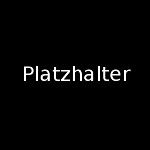
\includegraphics[scale=1.0]{spacer}
		\caption{Octree Darstellung - nach paper Hornung et al.}
		\label{fig.octree}
	\end{center}
	%\vspace*{-8mm}
\end{figure}


Die Besonderheit des von Hornung \textit{et al.} entwickelten Ansatzes liegt darin, dass im Gegensatz zu einer binären Darstellung der Voxelzustände eine probabilistische Bewertung vorgenommen wird. Es können somit bei der Betrachtung der Voxel mehr als zwei Zustände unterschieden werden, so dass zwischen belegten, freien und unbekannten Bereichen differenziert werden kann. Als Grenzwert der Verfeinerung kann eine anwendungsabhängige Auflösung definiert werden. Auch die Kombination verschiedener Strukturbäume mit unterschiedlichen Auflösungen ist bei der Verwendung von \textit{Octomap} möglich. Bei Bedarf können so bestimmte Strukturen feiner aufgelöst werden um die Genauigkeit der Abbildung zu erhöhen.\\
Einen Vergleich zwischen Modellumgebung und der daraus erzeugten \textit{Octomap} zeigt \abb{fig.octomap}.

\begin{figure}[!ht]
	\begin{center}
		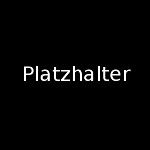
\includegraphics[scale=1.0]{spacer}
		\caption{Vergleich - Octomap Modellumgebung (Pointcloud)}
		\label{fig.octomap}
	\end{center}
	%\vspace*{-8mm}
\end{figure}

\section{Ermittlung der Initialpose}
\label{chap.globloc}
Für die globale Lokalisation wurde in dieser Arbeit ein Ansatz gewählt, welcher auf dem Monte Carlo Algorithmus basiert \cite{Dellaert1999}. Dieser Ansatz entspricht wie bereits in \abschnitt{chap:mcl} beschrieben einem Partikelfilter. Dazu wurde eine Implementierung \cite{humanoidNavigation} verwendet, welche das Lokalisationsverfahren innerhalb einer ROS-Node bereitstellt. Als Referenz wird die zuvor beschriebene aus der Modellumgebung erzeugte \textit{Octomap} verwendet. \red[Entwickelt für die Lokalisation eines humanoiden Roboters konnte die Implementierung so angepasst werden, dass sie auch die Lokalisation eines handgeführten Systems ermöglicht.]\\
In der vorhandenen Umgebungskarte werden dabei im Rahmen zuvor festlegbarer Parameter Partikel basierend auf einer Zufallsverteilung generiert. Jeder Partikel entspricht einer möglichen Pose des Kamera-Projektor-Systems und verfügt demnach über sechs Freiheitsgrade. Die Bestimmung der Pose des Kamera-Projektor-Systems erfolgt durch Auswertung der Partikel basierend auf einer Wahrscheinlichkeitsverteilung. Die Wahrscheinlichkeiten können dabei auf Basis zweier verschiedener Modelle berechnet werden: dem Endpoint-Modell und dem Raycasting-Modell. Da sich beide Modelle bei der Berechnung der Wahrscheinlichkeiten auf die Log-Likelihood-Funktion stützen soll diese zunächst kurz erläutert werden, bevor anschließend die beiden Modelle ausführlicher dargestellt werden.

\subsection{Log-Likelihood-Funktion}
\label{chap.loglik}
Ideale Entfernungsmesser würden bei einer Messung die exakten Distanzen zu den Hindernissen in ihrem Messbereich ermitteln. In der Realität sind jedoch alle Messungen mit einem Fehler durch lokales Messrauschen behaftet, welches im Fall des Kinect Sensors als Gaußverteilung modelliert werden kann \cite{Nguyen2012}. Es wird nun die Pose $\vek{x}{}{t}$ eines Partikels innerhalb der Karte $m$ betrachtet. Die Wahrscheinlichkeit $p$, ob ein Messwert $d_m^i$ aus einem bekannten Hindernis in der Entfernung $d_k$ resultiert lässt sich somit innerhalb des Intervalls der Sensorreichweite $[d_{min};d_{max}]$ über eine Verteilung mit Mittelwert $d_k$ und der Varianz des Sensors $\sigma_{S}^2$ ermitteln \cite{Thrun2005}:

\begin{equation}
p(d_m^i|\vek{x}{}{t},m) = \left\lbrace\begin{array}{ll}
\eta \: \mathcal{N}(d_m^i;d_k,\sigma_S^2) & \quad \mathrm{wenn} \quad d_{min}\leq d_m^i \leq d_{max} \\
0 & \quad \mathrm{sonst}
\end{array}
\right.
\end{equation}
Dabei ist $\eta$ ein für die verwendeten Modelle konstanter Normalisierungsfaktor und die Gaußverteilung mit der Differenz der Distanzen $\Delta d = d_m^i-d_k$  gegeben durch:

\begin{equation}
\mathcal{N}(d_m^i;d_k,\sigma_S^2) = \frac{1}{\sqrt{2\pi\sigma_S^2}} \; e^{-\dfrac{1}{2}\dfrac{{(\Delta d})^2}{\sigma_S^2}}
\end{equation}

Die Bestimmung der Wahrscheinlichkeit einer Pose erfolgt durch Betrachtung aller $n$, im Vektor $\vek{d}{}{m}$ zusammengefassten, Messwerte. Dazu wird angenommen, dass die Messwerte voneinander unabhängig sind und das Produkt der einzelnen Wahrscheinlichkeiten gebildet \cite{Hornung2010}. Dies ergibt die Likelihood-Funktion:

\begin{equation}
\label{eq.likelihood}
p(\vek{d}{}{m}|\vek{x}{}{t},m) = \prod_{i=1}^{n}p(d_m^i|\vek{x}{}{t},m)
\end{equation}

Durch Anwendung des natürlichen Logarithmus auf \eq{eq.likelihood} vereinfacht sich die Berechnung zur Bildung der Summe über die Messwerte:

\begin{equation}
\begin{split}
\log \: p(\vek{d}{}{m}|\vek{x}{}{t},m) & = \sum_{i=1}^{n}\log\: p(d_m^i|\vek{x}{}{t},m) \\[1em]
& = \sum_{i=1}^{n}\log \left( \frac{1}{\sqrt{2\pi\sigma_S^2}} \; e^{-\dfrac{1}{2}\dfrac{{(\Delta d})^2}{\sigma_S^2}} \right)\\[1em]
& = \underbrace{-\frac{1}{2}\log(2\pi\sigma_S^2)}_K-\dfrac{\sum_{i=1}^{n}(\Delta d)^2}{2\sigma_S^2}
\end{split}
\end{equation}
Da der natürliche Logarithmus eine streng monotone Funktion ist, bleibt die Stelle des Maximums der Ursprungsfunktion erhalten. Das bedeutet, der Partikel mit maximalem Wahrscheinlichkeitswert bleibt erhalten. Da die Partikel bei jeder Lokalisation lediglich relativ untereinander verglichen werden hat dieser Schritt keine Auswirkungen auf das Ergebnis. Die Konstante $K$ ist bei gleichbleibender Varianz für alle Messungen identisch und kann daher vorab berechnet werden.\\
Die so bestimmte Wahrscheinlichkeit der betrachteten Pose kann nun als Gewichtung verwendet werden um das Maximum über alle Partikel zu bestimmen. 

\red[Anpassung der Varianz in Abhängigkeit der Entfernung als Ausblick]

\subsection{Endpoint-Modell}
Das Endpoint-Modell, welches von \red[X] in \cite{Endpoint} beschrieben wurde, bestimmt die Wahrscheinlichkeit einer Pose anhand eines Distanz-Modells. Basierend auf der für die Lokalisation verwendeten \textit{Octomap} wird zunächst eine Lookup-Table erstellt, welche die räumlichen Dimensionen der Ausgangskarte abbildet. Jedem Voxel wird dabei ein Distanzwert zugewiesen, basierend auf der Entfernung zum nächsten Hindernis. Als Hindernisse gelten dabei alle belegten Zellen der \textit{Octomap}, also neben dem Raum auch alle in der Karte vorhanden statischen Objekte. Erfolgt die Lokalisation wie in dieser Arbeit innerhalb einer statischen Umgebung kann die Berechnung der Distanzkarte bereits vor der Lokalisation erfolgen.\\

\begin{figure}[!ht]
	\begin{center}
		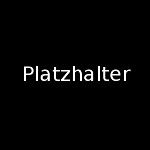
\includegraphics[scale=1.0]{spacer}
		\caption{Distance Map}
		\label{fig.dist_map}
	\end{center}
	%\vspace*{-8mm}
\end{figure}

Durch die vorhergehende Berechnung dieser Karte ergibt sich eine deutliche Verringerung des Rechenaufwands bei jedem Lokalisationsschritt. Anzumerken bleibt, dass die Distanz-Karte während der gesamten Programmlaufdauer im Speicher behalten wird und bezüglich des Speicherbedarfs die Ausgangskarte deutlich übersteigen kann.\\
Die Lokalisation erfolgt beim Endpoint-Modell durch Betrachtung der Punkte der Punktewolke. Diese werden als Endpunkte der Strahlen interpretiert, welche von der Kamera an der jeweiligen Partikelpose ausgesendet werden. Durch Abbildung auf die zuvor berechnete Distanz-Karte können die darin gespeicherten Werte für $\Delta d$ ausgelesen werden. Die Wahrscheinlichkeiten, dass die Punktwolke von der Stelle des betrachteten Partikels aus aufgenommen wurde lässt sich anschließend anhand der Distanzwerte bestimmen. Die berechneten Wahrscheinlichkeiten aller Strahlen werden innerhalb der unter \abschnitt{chap.loglik} beschriebenen Log-Likelihood-Funktion addiert um den Partikel mit der höchsten Gewichtung zu ermitteln.\\
Das Endpoint-Modell bildet nicht direkt die physikalische Arbeitsweise eines Entfernungsmessers ab, da es durch Hindernisse \glqq hindurchsehen\grqq{} kann, wie \abb{fig.endpoint} zeigt. Dennoch ist es in der Lage, eine zuverlässige Approximation der Systempose zu bestimmen \cite{Konolige1999}.\\

\red[An welcher Stelle?: Die Bestimmung erfolgt mittels der Log-Likelihood-Funktion, welche eine statistische Aussage über die Wahrscheinlichkeit der Messung berechnet.\\]

\begin{figure}[!ht]
	\begin{center}
		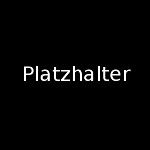
\includegraphics[scale=1.0]{spacer}
		\caption{Endpoint-Modell}
		\label{fig.endpoint}
	\end{center}
	%\vspace*{-8mm}
\end{figure}

\subsection{Raycasting-Modell}
Beim Raycasting Modell, welches ebenfalls\red[oder andere quelle?] von X in \cite{Raycasting} beschrieben wird, werden für jede Pose nicht die Endpunkte der ausgesendeten Strahlen betrachtet, sondern ihr Verlauf. Entlang der Strahlen von der Kamera zu den Messpunkten der aufgenommenen Punktwolke findet ein Abgleich mit den Daten der Karte statt. Erreicht der Strahl einen besetzen Bereich in der Karte endet die Betrachtung wie in \abb{ref.raycast} dargestellt.\\

\begin{figure}[!ht]
	\begin{center}
		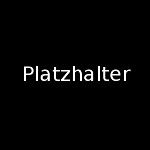
\includegraphics[scale=1.0]{spacer}
		\caption{Raycasting-Modell}
		\label{fig.raycast}
	\end{center}
	%\vspace*{-8mm}
\end{figure}

Die Entfernung zwischen dem ermittelten Punkt und dem betrachteten Partikel wird berechnet und anschließend mit der Entfernung des zugehörigen Sensorwertes verglichen. Die Differenz $\Delta d$ der beiden Distanzen wird anschließend verwendet um die Wahrscheinlichkeit zu bestimmen, dass der Sensorwert an dieser Stelle aufgenommen wurde. Die Berechnung der jeweiligen Wahrscheinlichkeit erfolgt dabei wie auch beim Endpoint-Modell mittels der Log-Likelihood-Funktion.\\

Zusätzlich wurde eine Root Mean Square (RMS) Berechnung der Distanzen implementiert. Die Ergebnisse korrelieren aufgrund der zugeordneten Wahrscheinlichkeiten bei fehlenden Distanzwerten nicht exakt mit den berechneten Wahrscheinlichkeitswerten, erlauben jedoch eine Bewertung der Güte der Anpassung zwischen Karten- und Sensordaten. Im Gegensatz zu den absoluten Gewichten der Partikel bietet dieses Maß damit eine Möglichkeit Lokalisationen mit unterschiedlichen Modellparametern zu vergleichen.\\

\red[Markerbasierte Lokalisation\\]
\red["Tracking" durch Verringerung der Partikelanzahl möglich, da sich die Rechenzeit deutlich verringert]



\section{Verfolgung der aktuellen Pose}
\label{locloc}
Im Anschluss an die globale Lokalisation wird die Bewegung des Systems kontinuierlich verfolgt und die aktuelle Pose aktualisiert. Da das handgeführte System nicht über Odometriedaten verfügt, wie sie beispielsweise bei einem mobilen Robotersystem durch Messungen der Radumdrehungen zur Verfügung stehen, muss das Tracking auf Basis anderer Eingangswerte durchgeführt werden. Dazu wird die unter \abschnitt{chap.visodom} aufgeführte visuelle Odometrie eingesetzt und eine Fusionierung mit den Daten der inertialen Messeinheit durchgeführt.\\

\subsection{Visuelle Odometrie}
Die visuelle Odometrie basiert auf den Bilddaten des Kinect Sensors. Neben dem Farbbild wird auch die aus dem Infrarotbild bestimmte Tiefenkarte ausgewertet. Dabei wird eine Implementierung \cite{Fovis} eingesetzt, welche die visuelle Odometrie unter dem Namen FOVIS als quell-offene Bibliothek für ROS bereitstellt.\\
Die Bestimmung der visuellen Odometrie erfolgt dabei in sechs aufeinanderfolgenden Schritten \cite{Huang2011}:

\begin{enumerate}
\item Das Farbbild wird in ein Grauwertbild konvertiert und mittels eines Gauß-Kernels\red[erklären?] geglättet. Es wird außerdem eine Gauß-Pyramide\red[footnote?] angelegt, um eine robustere Detektion der Bildmerkmale zu ermöglichen.
\item Innerhalb jeder Ebene der Gauß-Pyramide wird eine Merkmalserkennung mit adaptivem Schwellwert durchgeführt. Alle Merkmale ohne korrespondierende Informationen innerhalb des Tiefenbildes werden an dieser Stelle verworfen.
\item Anhand des aktuellen und des vorangegangenen Bildes wird eine initiale Approximation der Rotation des Systems durchgeführt, um den Suchbereich für anschließende Merkmalsextraktionen eingrenzen zu können. An dieser Stelle ist anzumerken, dass diese Methode für den Anwendungsfall eines autonomen, fliegenden Systems ausgelegt ist. Da ein handgeführtes System jedoch die gleichen Freiheitsgrade besitzt kann das Verfahren ohne Einschränkungen genutzt werden.
\item Den extrahierten Merkmalen wird ein Deskriptor zugewiesen, welcher einen Vergleich der Merkmale innerhalb aufeinander folgender Bilder ermöglicht. Durch Minimierung der Fehlerquadrate der zueinander passenden Deskriptoren kann anschließend die Lokalisation des Merkmals verfeinert und somit ein Abgleich im sub-pixel Bereich durchgeführt werden.
\item Um die Plausibilität zu überprüfen und falsch erkannte Merkmale zu eliminieren wird ein Vergleich der Merkmale zwischen den Bildern durchgeführt. Ausgehend von der Annahme, dass es sich um eine statische Szene handelt, kann dazu die euklidische Distanz zwischen den Positionen der Merkmale verwendet werden.
\item Für die finale Bestimmung der Odometrie des Systems wird zunächst die Transformation zwischen den Posen der aufgenommenen Bilder durch Minimierung der euklidischen Distanzen zwischen den verbliebenen Merkmalen bestimmt. Durch eine Minimierung des Rückprojektionsfehlers wird diese Transformation anschließend verfeinert. Eine weitere Verfeinerung kann erfolgen, falls Merkmale aufgrund eines zu großen Fehlers in der Rückprojektion aus der Betrachtung entfernt werden.
\end{enumerate}
Die visuelle Odometrie liefert durch das beschrieben Verfahren ein Ergebnis für die Veränderung der aktuellen Pose bezüglich aller sechs Freiheitsgrade. \abb{ref.fovis} \red[(c)] zeigt die aus zwei aufeinander folgenden Bildern ermittelte Veränderung der Pose anhand der Merkmale.\\
Um eine höhere Genauigkeit zu erreichen werden ergänzend die Messdaten einer inertialen Messeinheit betrachtet.

\begin{figure}[!ht]
	\begin{center}
		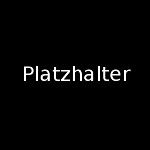
\includegraphics[scale=1.0]{spacer}
		\caption{Fovis \red[subfigures: RGB Bild - Tiefenbild - Merkmale]}
		\label{fig.fovis}
	\end{center}
	%\vspace*{-8mm}
\end{figure}

\subsection{Inertiale Messeinheit}
Die in \abschnitt{chap.imu} beschriebene inertiale Messeinheit ist in der Lage die translatorischen und rotatorischen Beschleunigungen des Systems zu messen. Auf Basis des von Mahony \textit{et al.} \cite{Mahony2008} entwickelten Algorithmus wird aus den Messdaten die Orientierung der Messeinheit bestimmt. Die verwendete Implementierung für den Arduino Nano (\abschnitt{chap.arduino}) zur Anbindung an das System basiert auf \cite{IMUCode}. Um die Messdaten in die Softwareimplementierung einzubinden wurde eine Schnittstelle für ROS ergänzt. Darüber hinaus wurde eine Gravitationskompensation implementiert, welche neben der Verwendung des Roll- und Nickwinkels auch das Auslesen der relativen Beschleunigungen des Systems ermöglicht.\\
Als Ergänzung der visuellen Odometrie werden die Messdaten der inertialen Messeinheit mit den Odometriedaten mittels eines Erweiterten Kalman-Filters fusioniert.

\subsection{Erweitertes Kalman Filter}
Das Kalman-Filter stellt eine in der Praxis bewährte Methode zur Fusionierung von Sensordaten dar. Es handelt sich beim Kalman-Filter \cite{Kalman1960} um die spezielle Implementierung eines Bayes-Filters, welcher eine statistische Approximation des aktuellen Systemzustands ermöglicht. Der Ausgang jeder auf ein System wirkende Aktion, beispielsweise die Drehung der Räder, kann in der Realität nicht ohne Unsicherheiten vorhergesagt werden. Der neue Systemzustand ist deshalb allein auf Basis der Odometriedaten nur mit großer Varianz bestimmbar. Messungen können dazu verwendet werden, diese Unsicherheiten zu korrigieren um den realen Zustand mit höherer Genauigkeit schätzen zu können. Die Besonderheit des Kalman-Filters liegt darin, dass die Unsicherheiten der Messungen und Aktionsresultate durch Gaußverteilungen mit dem Erwartungswert $\mu$ und der Standardabweichung $\sigma$ modelliert werden \cite{Hertzberg2012}. \abb{fig.kalman}\red[in anlehung an Hertzberg s.134] zeigt das Prinzip der Zustandsannäherung und die auf Basis der Messwerte durchgeführte Korrektur.\\
Durch das Erweiterte Kalman-Filter (EKF) kann dieses Filterprinzip durch Linearisierung der Systemzustände auch auf nichtlineare Systeme angewendet werden. In dieser Arbeit wurde eine Implementierung des EKF verwendet \cite{EKF}, welche eine direkte Anbindung an ROS zur Verfügung stellt. Die auf das handgeführte System einwirkenden Aktionen, insbesondere also die Bewegung des Systems durch den Anwender, werden dabei durch die verwendete visuelle Odometrie detektiert. Mit Hilfe der inertialen Messeinheit kann die bestimmte Systempose aktualisiert und verfeinert werden. Dabei werden neben den absoluten Werten des Roll- und Nickwinkels auch die Beschleunigungen bezüglich der drei Systemachsen integriert um die Bewegung des Systems zu schätzen.


\red[odometrie auch Messung...Varianz der -sensoren aber klein gegenüber dem Umgebungseinfluss]
Partikelbasiertes Tracking\\
Featurebasiertes Tracking\\
Beschleunigungsdatenbasiertes Tracking\\
Kombination der Odometriedaten durch Extended Kalman Filter \red[Buch Hertzberg]\\
\red[Ergebnisse der Kalman Einbindung mit und ohne IMU auswerten]
\red[Fovis differential auf true und imu auf false?]